\subsection{Impact of activation function on validation accuracy}
\label{subsection:experiments:classification:activation}
Since the activation function gives rise to nonlinearity, it is reasonable to conjecture that the activation function affects performance. In \nameref{chapter:literature-review} and \nameref{chapter:universality}, we have also observed that the properties of activation function also play an essential role in many proofs of universality.

To begin an experimental study of the effects of the activation function, we will focus on neural networks with a single hidden layer. Each neural network is trained using the configuration from Table \ref{table:expriments:training_config}. In this experiment, only the hidden layer width and the activation function are varied. For each experiment configuration, the model achieving the best validation accuracy is saved and used in the following analysis.

According to the results displayed in Figure \ref{fig:experiments:classification:all-activations-plot}, it is likely that the activation function significantly affects validation set accuracy, given current training configuration. Thus, it is reasonable to conjecture that the activation function affects the generalization error. It is interesting to note that sigmoid and $\tanh$ significantly and consistently outperform $\operatorname{ReLU}$ regardless of hidden layer width. That is slightly surprising because many modern neural network architectures use $\operatorname{ReLU}$ and similar rectified activation functions instead of $\operatorname{sigmoid}$ and $\tanh$.

It can be shown that $\operatorname{sigmoid}$  and $\tanh$ are algebraically related. More precisely, for every $x \in \R, \tanh{(x)} = 2\sigma(2x) - 1$. Given the structure of a fully-connected neural network and this algebraic connection, it is reasonable to expect that $\operatorname{sigmoid}$  and $\tanh$ produce similar results. According to the results displayed in Figure \ref{fig:experiments:classification:all-activations-plot}, that is indeed the case. Another surprising observation is the significant validation accuracy drop for $\operatorname{ReLU}$ networks after hidden layer width of 128 neurons. Although ReLU networks perform worse as the hidden layer width increases, it seems that $\operatorname{sigmoid}$ and $\tanh$ networks perform better. The widest $\tanh$ and $\operatorname{sigmoid}$ achieve the best validation accuracy. We will briefly discuss the worst $\operatorname{ReLU}$ model. According to the Figure \ref{fig:experiments:classification:wide-relu-plot}, validation and test accuracy are consistently very similar. Hence, there is no evidence of overfitting.

\begin{figure}[H]
    \begin{minipage}{.5\textwidth}
        \centering
        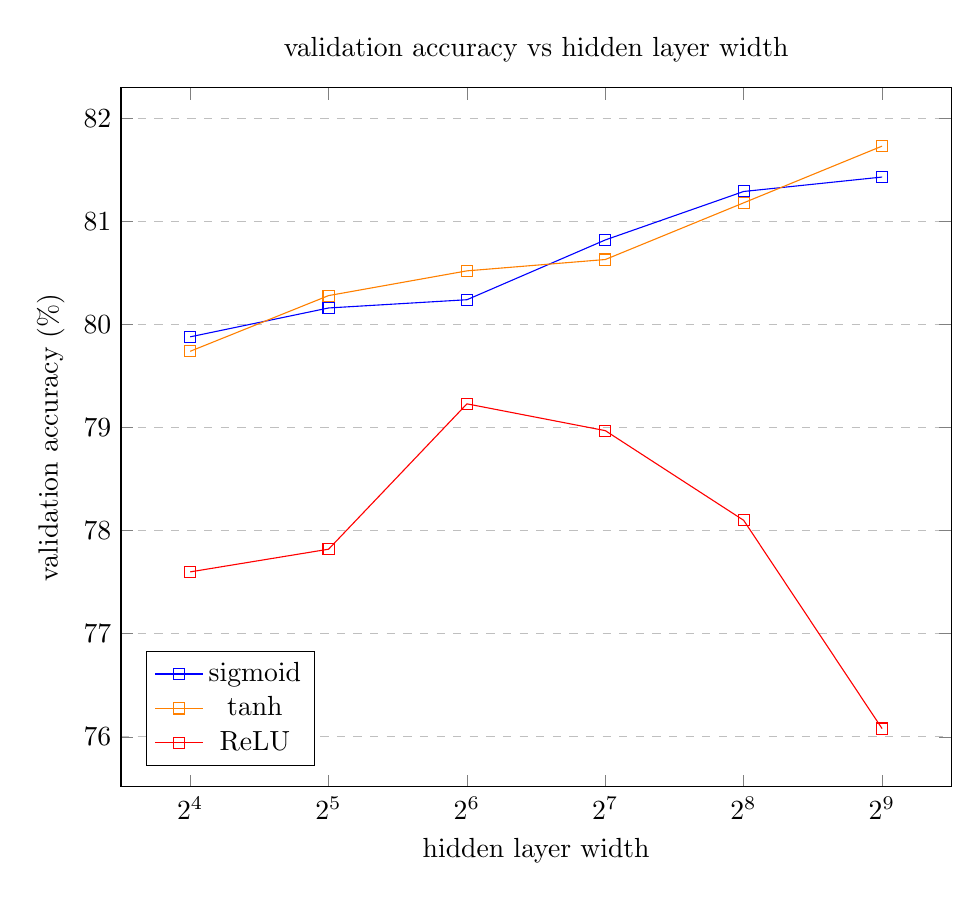
\begin{tikzpicture}
            \begin{axis}[
                width=\textwidth,
                title={validation accuracy vs hidden layer width},
                xlabel={hidden layer width},
                ylabel={validation accuracy (\%)},
                ymajorgrids=true,
                grid style=dashed,
                xmode=log,
                legend pos=south west,
                log basis x={2}]
                \addplot[mark=square,blue] coordinates {(16,79.88) (32,80.16) (64,80.24) (128,80.82) (256,81.29) (512,81.43)};
                \addplot[mark=square,orange] coordinates {(16,79.74) (32,80.28) (64,80.52) (128,80.63) (256,81.18) (512,81.73)};
                \addplot[mark=square,red] coordinates {(16,77.60) (32,77.82) (64,79.23) (128,78.97) (256,78.10) (512,76.08)};
                \legend{sigmoid, tanh, ReLU}
            \end{axis}
        \end{tikzpicture}
        \captionof{figure}{Validation accuracy of the best model with given hidden layer width and activation function}
        \label{fig:experiments:classification:all-activations-plot}
    \end{minipage}%
    \hspace{0.5cm}
    \begin{minipage}{.5\textwidth}
        \centering
        \includegraphics[scale=0.5]{experiments/classification/relu-single-layer-no-overfitting.png}
        \captionof{figure}{Training and validation accuracy of $\operatorname{ReLU}$ network with a single hidden layer of 512 neurons. This is the worst $\operatorname{ReLU}$ model in this experiment.}
        \label{fig:experiments:classification:wide-relu-plot}
    \end{minipage}
\end{figure}

